\chapter{Accelerator Design and Optimisation Methods}
\label{ch:design}

\section{Design Philosophy and Architecture}

The accelerator was shaped by the execution structure of CSR SpMM rather
than adapted from a generic dense-matrix template. CSR SpMM has three
distinct computational phases (row-bound loading, nonzero streaming, and
dense tile accumulation), and each phase has a different memory and
control-flow character. Any hardware design that treats them as a single
monolithic pipeline inevitably over-engineers one phase and underserves
another, so the architecture instead separates concerns explicitly: a
control finite state machine (\texttt{accel\_ctrl}) walks the CSR structure
and sequences RAM accesses, while a datapath (\texttt{accel\_datapath})
performs the parallel multiply--accumulate and manages the local tile
buffers. This split follows standard digital design
practice~\citep{sze2017} and, more importantly, allows each half of the
accelerator to be verified independently in simulation before integration.

The top-level module (\texttt{accel\_top}) wraps these two blocks together
with an MMIO front-end that decodes the PicoRV32 memory bus and exposes the
configuration interface of Table~\ref{tab:mmio-regs}. The accelerator
reaches shared memory through Port~B of the dual-port BRAM, a 32-bit
word-granular port with one cycle of registered read latency. All RAM
accesses are therefore scheduled as paired issue/consume phases separated
by exactly one clock cycle, which gives the controller a deterministic
latency model and removes the need for a stall/ready handshake.

\section{Baseline Datapath}

The datapath is parameterised by a tile width $TN = 8$ (the number of
output columns processed in parallel), a maximum row count
$M_{\mathrm{max}} = 64$, and a 32-bit signed operand width. Its behaviour
depends on two local buffers whose sizing is critical to performance. The
first, \texttt{B\_Seg}, is an eight-element array of signed 32-bit values
that holds the current row segment of dense matrix $B$: for every nonzero
$a_{ij}$ the controller fills \texttt{B\_Seg} with
$B[j,\,c_0:c_0{+}TN]$ before enabling the MAC array. The second,
\texttt{C\_Tile}, is an $M_{\mathrm{max}} \times TN$ array of signed 32-bit
partial sums that accumulates the output tile for all rows of $C$
simultaneously within the current tile column $[c_0, c_0{+}TN)$. Using a
flat two-dimensional accumulator rather than per-row registers avoids
writeback/restore cycles when nonzeros from different rows touch the same
tile column, which is the common case in realistically distributed sparse
matrices. The C-tile is implemented as a 512-register fabric array rather
than BRAM; on the Cyclone~V each ALM carries two registers, so the tile
consumes roughly 256 ALMs, well within the budget of the target device.

For each nonzero $a = A[i,k]$ the controller asserts \texttt{mac\_en},
\texttt{mac\_row} $= i$, and \texttt{mac\_a} $= a$, and the datapath issues
eight simultaneous signed multiply--accumulate operations:
\[
  \texttt{C\_Tile}[i][c] \;\mathrel{+}=\; \texttt{mac\_a} \,\times\,
  \texttt{B\_Seg}[c] \qquad c = 0, 1, \ldots, TN{-}1.
\]
This is the key mapping that gives the accelerator its parallelism: a
single nonzero in $A$ interacts with an entire row segment of $B$, so one
issue cycle produces $TN$ output updates. The parallelism is across the
dense output dimension, where the workload is regular, rather than along
the sparse dimension, where it is not. When all rows have been processed
in the current tile column, the C-tile is streamed back to shared RAM row
by row; if \texttt{CTRL.relu\_en} is asserted, an element-wise
$\max(0, \cdot)$ is applied to each value on writeback, making the
accelerator directly usable as the fully-connected layer of a neural
network inference pipeline.

\section{Control FSM}
\label{sec:fsm}

The control FSM is the most intricate component of the design. It drives
all address generation, RAM sequencing, nonzero traversal, and tile
management, and cycles through the phases listed in
Table~\ref{tab:fsm-states}; the sub-phase indices within
\texttt{ROW\_LOAD} and \texttt{NZ\_FETCH} exist specifically to cover the
one-cycle registered RAM latency. The simplified state-level view is
shown in Figure~\ref{fig:accel-fsm}.

\begin{table}[htbp]
  \centering
  \small
  \begin{tabular}{p{3.8cm}p{8.6cm}}
  \toprule
  State & Action \\
  \midrule
  \texttt{IDLE} &
    Wait for \texttt{start} pulse. Load $M$, $N$, $K$, NNZ, and base
    addresses from the MMIO register snapshot. \\[4pt]
  \texttt{INIT\_TILE\_CLEAR} &
    Clear all entries of \texttt{C\_Tile} to zero in preparation for the
    first tile column (one row per cycle, $M_{\mathrm{max}}$ cycles). \\[4pt]
  \texttt{ROW\_LOAD} &
    Load the CSR row bounds for the current row $i$: issue reads for
    \texttt{rowptr[i]} and \texttt{rowptr[i+1]}; handle the registered RAM
    output latency using sub-phases \texttt{ROW\_PHASE\_0/1/2}. \\[4pt]
  \texttt{NZ\_FETCH} &
    For each nonzero in \texttt{[rowptr[i], rowptr[i+1])}: read
    \texttt{values[p]} and \texttt{colidx[p]} and compute the starting
    address of $B[\texttt{col},:]$ for the current tile. Sub-phases
    \texttt{NZ\_PHASE\_0}--\texttt{NZ\_PHASE\_4} handle RAM latency and
    address arithmetic. \\[4pt]
  \texttt{MAC} &
    Fill \texttt{B\_Seg} with $TN$ consecutive values from $B$ (one per
    clock in INT32 mode, two reads total in INT8 mode), then assert
    \texttt{mac\_en} for one cycle to update \texttt{C\_Tile}. \\[4pt]
  \texttt{NEXT\_ROW} &
    Increment the row index. If more rows remain in this tile column, loop
    to \texttt{ROW\_LOAD}; otherwise proceed to \texttt{WRITE\_TILE}. \\[4pt]
  \texttt{WRITE\_TILE} &
    Write all $M \times TN$ entries of \texttt{C\_Tile} back to shared RAM
    (with optional ReLU). Advance the tile column offset by $TN$; if more
    tile columns remain, clear \texttt{C\_Tile} and loop to
    \texttt{ROW\_LOAD}, otherwise proceed to \texttt{DONE}. \\[4pt]
  \texttt{DONE} &
    Assert \texttt{STATUS.done} and release \texttt{STATUS.busy}; return
    to \texttt{IDLE} when \texttt{clear\_done} is asserted by the CPU. \\
  \bottomrule
  \end{tabular}
  \caption{Accelerator FSM states and their actions.}
  \label{tab:fsm-states}
\end{table}

\begin{figure}[htbp]
  \centering
  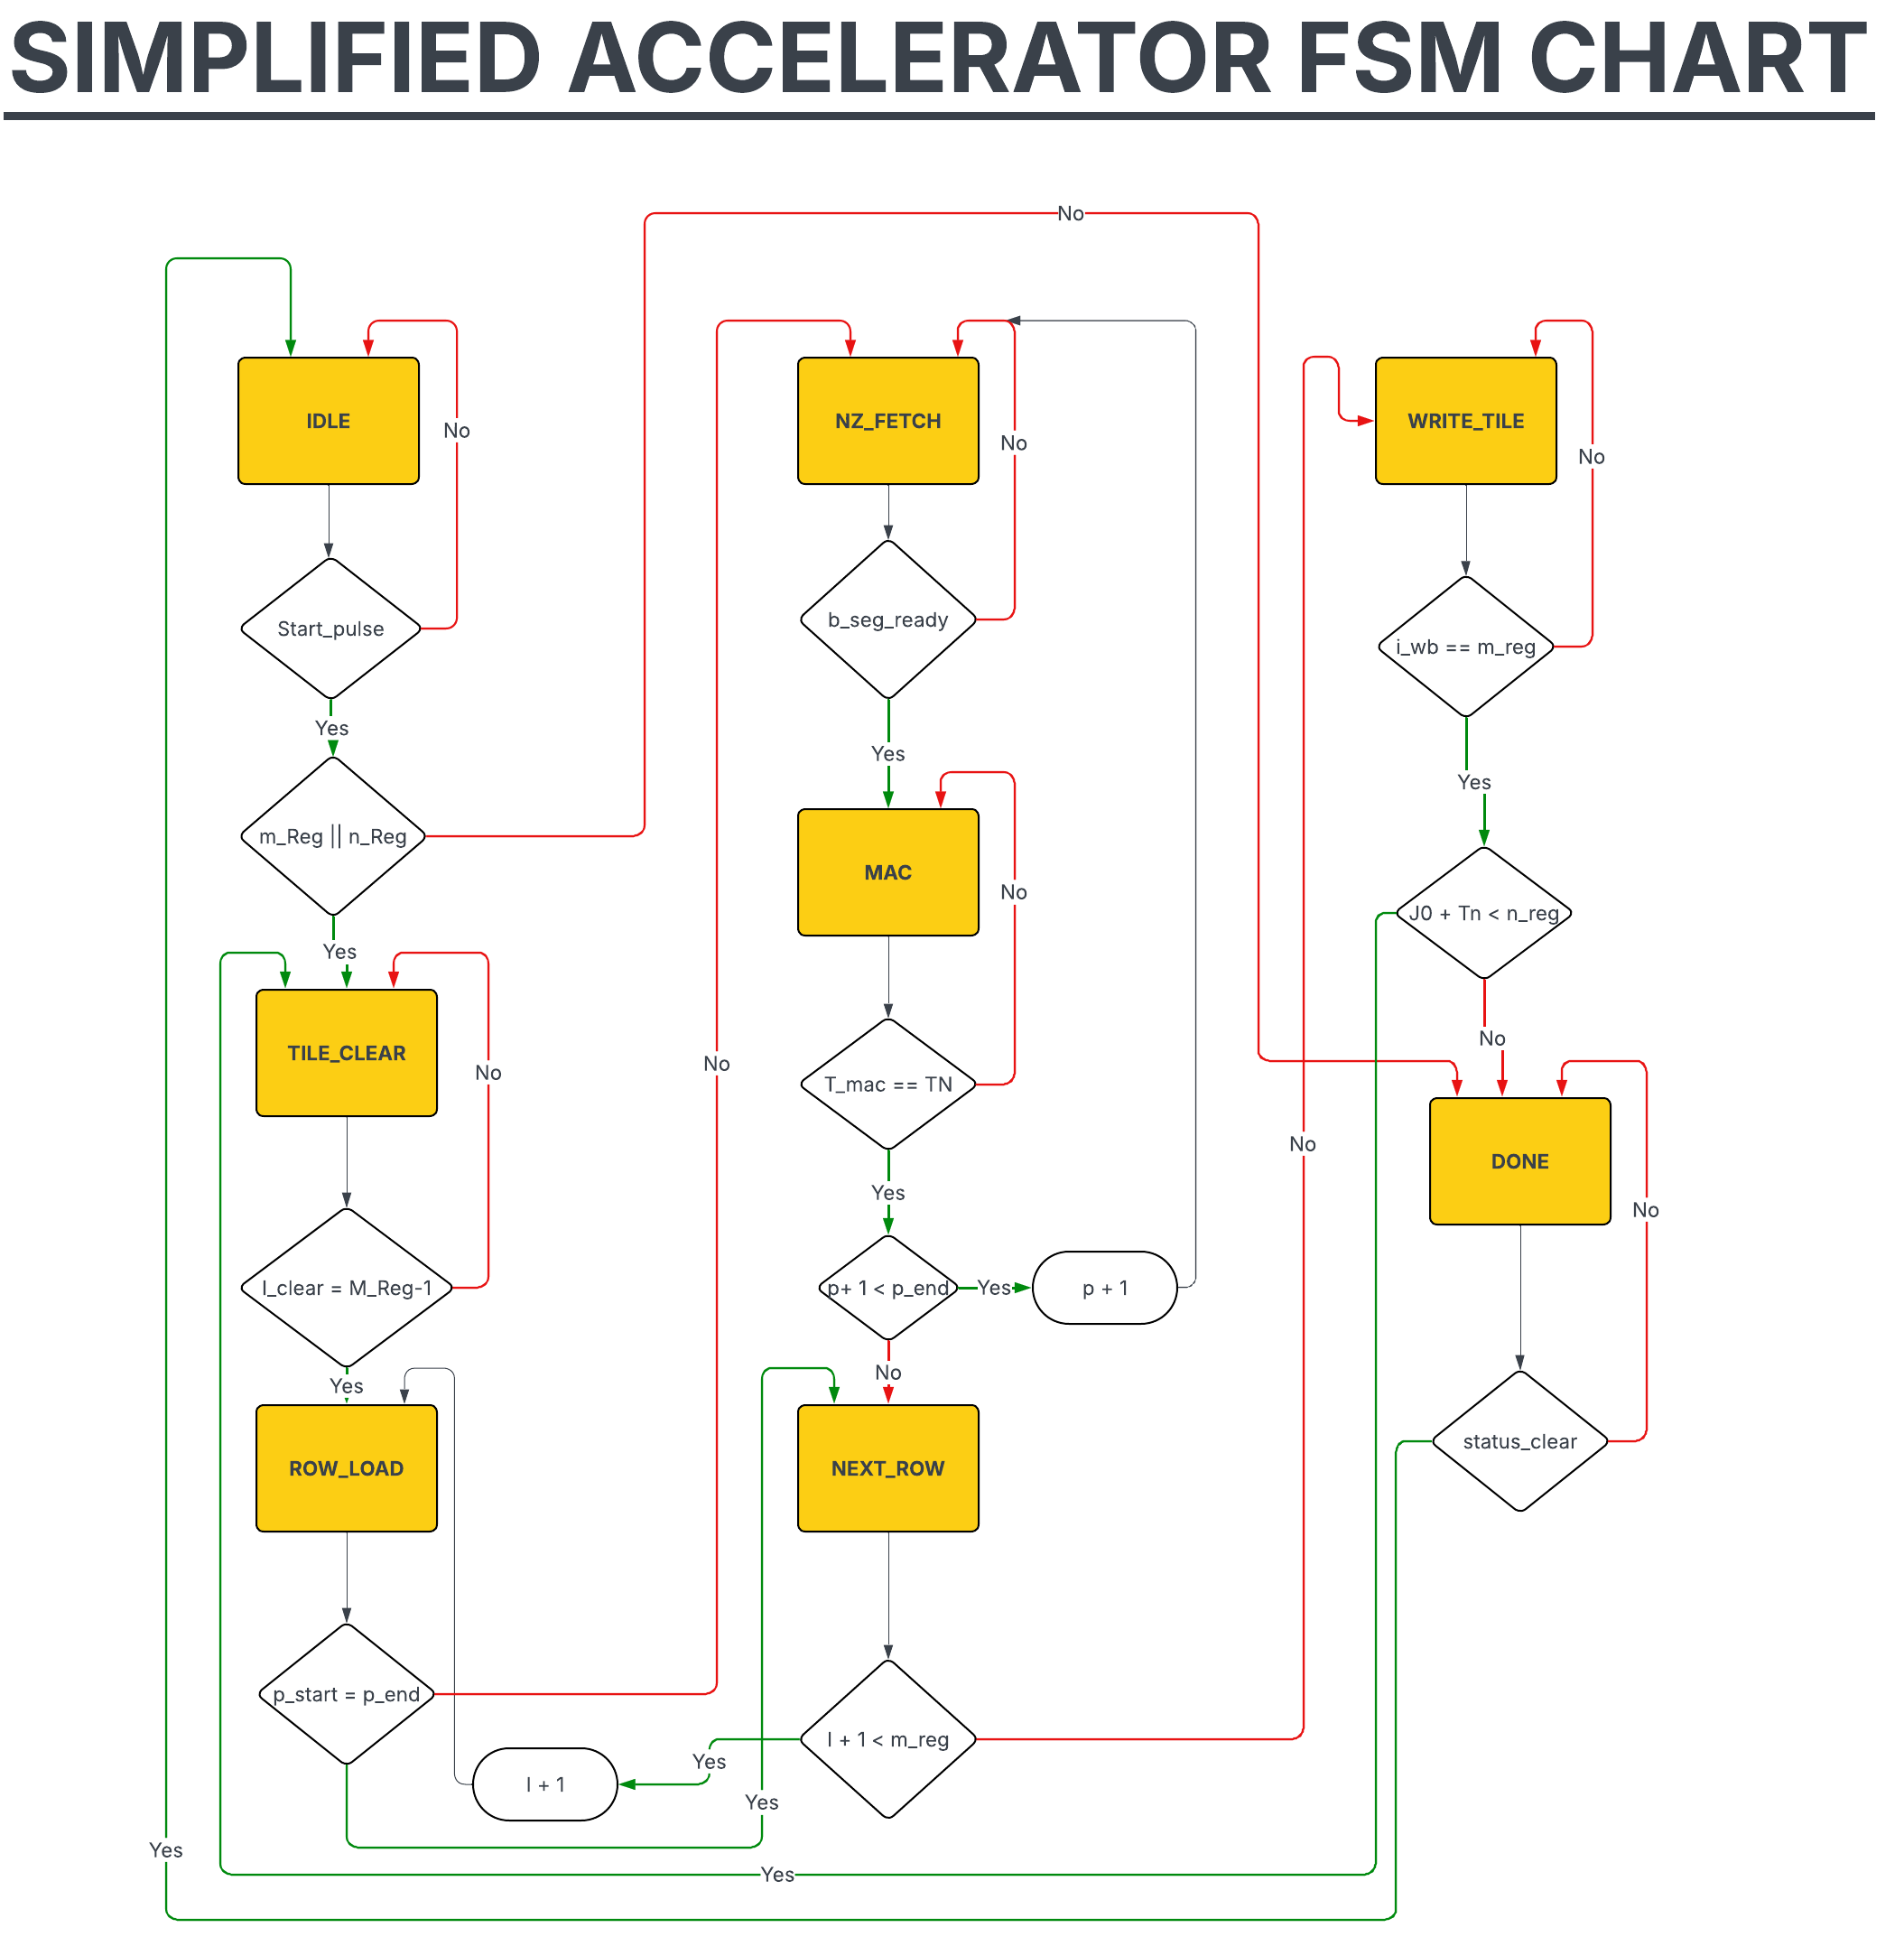
\includegraphics[width=\textwidth]{accel_fsm.png}
  \caption{Simplified accelerator finite state machine. Each major phase
           corresponds to one row in Table~\ref{tab:fsm-states}. Sub-phase
           transitions within \texttt{ROW\_LOAD} and \texttt{NZ\_FETCH}
           handle the one-cycle registered RAM output latency.}
  \label{fig:accel-fsm}
\end{figure}

For a matrix with $M$ rows, NNZ nonzeros, and dense width $N$ (processed
in $N/TN$ tile columns), the approximate cycle budget per tile column is
\[
  T_{\mathrm{tile}} \approx M_{\mathrm{max}} + M \cdot C_{\mathrm{row}}
  + \text{NNZ} \cdot (C_{\mathrm{nz}} + TN) + M \cdot TN \cdot C_{\mathrm{wb}},
\]
with $C_{\mathrm{row}} \approx 5$ cycles per row-bound load,
$C_{\mathrm{nz}} \approx 5$ cycles per nonzero fetch, and
$C_{\mathrm{wb}} \approx 1$ cycle per output writeback. At $TN = 8$ the
nonzero fetch and $B$-segment fill together contribute roughly
$5 + 8 = 13$ cycles per nonzero, and the reader will see directly how
shrinking the $TN$-dependent term is what the INT8 optimisation later
attacks.

\section{The Choice of Tile Width}
\label{sec:tn-choice}

The tile width $TN$ sets the degree of parallelism in the dense dimension,
and its selection is a balance between arithmetic throughput, register
array size, memory-access burden, and routing feasibility on the target
device. Table~\ref{tab:tn-tradeoffs} summarises the options. At $TN = 1$
the accelerator degenerates to a sequential MAC with no parallel benefit;
$TN = 4$ offers modest parallelism at the price of halving the reuse of
each fetched $B$ segment; $TN = 16$ or $TN = 32$ doubles or quadruples the
register array and the number of required DSP blocks, at which point both
routing congestion and timing closure become the limiting factor on a
Cyclone~V that already carries a CPU, BRAM, UART, and GPIO. A tile width
of eight maps cleanly onto eight DSP multiply--accumulate blocks, keeps
the 512-register C-tile within practical limits, and covers the smallest
benchmark width ($N = 8$) in a single tile column so no case in the suite
is penalised by tiling overhead. It was also the largest width that
consistently closed timing at 50\,MHz in preliminary synthesis, which
settled the choice for the final design.

\begin{table}[htbp]
  \centering
  \small
  \begin{tabular}{lccccp{3.8cm}}
  \toprule
  $TN$ & MAC lanes & Acc.\ registers & B-seg reads/NZ & DSP estimate & Notes \\
  \midrule
  1  & 1 & 64 & 1 & 1 &
    Minimal resources; no parallelism; effectively sequential. \\
  4  & 4 & 256 & 4 & 4 &
    Moderate parallelism; reduced register pressure. \\
  8  & 8 & 512 & 8 & 8 &
    \textbf{Design point.} Good balance; DSP-mappable; 512-reg array feasible. \\
  16 & 16 & 1024 & 16 & 16 &
    Doubles resources; increases routing congestion; timing harder to close. \\
  32 & 32 & 2048 & 32 & 32 &
    Likely infeasible on Cyclone~V; 2048-reg array exceeds practical limits. \\
  \bottomrule
  \end{tabular}
  \caption{Resource and performance implications of different tile widths
           $TN$. The accelerator implements $TN = 8$.}
  \label{tab:tn-tradeoffs}
\end{table}

\section{Algorithmic Decomposition: Row-Wise CSR Traversal}

The first and most consequential design decision was algorithmic: process
CSR rows serially and tile only the dense dimension. Alternatives such as
outer-product decomposition (as in OuterSPACE~\citep{outerspace2018}) or
intersection-based skipping (as in ExTensor~\citep{extensor2019}) can
deliver higher throughput in certain regimes, but they do so by introducing
index-merge networks, multi-port accumulation, and in some cases
content-addressable storage, none of which are feasible inside the SoC
budget of this project. Row-wise CSR traversal keeps the FSM tractable
enough to verify by hand, keeps the BRAM Port~B access pattern regular so
no bank conflicts arise, and keeps the C-tile writeback purely sequential
with no merge logic. The simplicity pays for itself in both correctness
confidence and timing-closure margin.

\section{Memory Optimisation: the B-Segment Bottleneck}

In the baseline configuration, filling \texttt{B\_Seg} for a single
nonzero requires $TN = 8$ consecutive 32-bit RAM reads. With the one-cycle
registered latency each fill therefore takes at least $TN + 1 = 9$ cycles,
and the subsequent MAC another cycle, so roughly ten cycles of useful work
accumulate per nonzero once the segment is in place. These reads dominate
the per-nonzero cost entirely, and any architectural improvement that
leaves them untouched is bounded in impact.

INT8 packing is the architectural lever that directly addresses the
bottleneck. With matrix $B$ stored as packed INT8 at four values per
32-bit word, two consecutive aligned 32-bit reads deliver all eight INT8
values required to fill a $TN = 8$ segment, and the hardware extracts the
individual bytes in a single combinatorial stage:
\begin{equation}
  \texttt{B\_Seg}[4k + b] = \mathrm{sign\_ext}_{8 \to 32}
  \!\left( \texttt{ram\_rdata}[8(b{+}1){-}1 : 8b] \right),
  \quad b \in \{0, 1, 2, 3\},
  \label{eq:byte-extract}
\end{equation}
where the selected byte is placed in the lower eight bits of a 32-bit
register and the upper 24 bits are filled with the sign of that byte.
The segment fill therefore drops from eight cycles to two, a $4\times$
reduction in the memory-bound component of the per-nonzero cycle budget,
with no additional pipeline stage and no change to accumulation precision.

\section{DSP-Oriented Parallel MAC Enhancement}

The second optimisation stage restructured the MAC array to increase the
fraction of DSP blocks utilised per cycle. On the Cyclone~V, each DSP
block implements an 18$\times$18-bit signed multiplier followed by a
dedicated accumulator register, but the synthesis tool maps RTL
multipliers onto these blocks only if the operand widths and
accumulation structure match the block's
configuration~\citep{intel_dsp_blocks}. In the baseline design the eight
MAC operations are described as generic 32-bit multipliers; depending on
register fan-out and routing pressure, Quartus may or may not pack them
into DSP blocks, and in practice some lanes were being inferred in ALM
logic.

The DSP MAC stage rewrites the multiply--accumulate explicitly in the
registered-feedback form that the tool recognises as DSP-friendly:
\[
  \texttt{C\_Tile}[i][c] \;\leftarrow\; \texttt{C\_Tile}[i][c] + a \cdot B[c],
\]
using 32-bit signed operands and a registered accumulator. With this
structure Quartus maps each of the eight MAC lanes independently onto a
dedicated DSP multiplier/accumulator block rather than inferring ALM-based
multiplier cascades, and the resulting design completes each MAC in one
clock cycle with less ALM logic and lower power dissipation. Across the
full 12-case benchmark sweep this stage reduced total accelerator offload
cycles from 427,299 to 324,568, a $1.32\times$ improvement. The modest
gain is itself the interesting result: it confirms that the baseline was
not limited by arithmetic execution, and that further attention has to be
paid to memory traffic if the speedup ceiling is to move.

\section{INT8 Mode at the Datapath Level}

When \texttt{CTRL.int8\_mode} is asserted, three specific aspects of the
datapath change. The CSR \texttt{values} array is now stored as packed
INT8, and the controller tracks the byte offset of the current nonzero
within its 32-bit word using a two-bit counter: for nonzero index $p$ the
byte offset is $b = p \bmod 4$ and the enclosing word lives at
\texttt{A\_VAL\_BASE} $+ \lfloor p/4 \rfloor \times 4$, from which the
same sign-extension circuit used for $B$-byte extraction
(Equation~\ref{eq:byte-extract}) recovers a full-precision 32-bit $a$
before multiplication. The $B$-segment fill is replaced with the two-read
path described in the previous section, filling all eight lanes of
\texttt{B\_Seg} in two cycles instead of eight. Accumulation itself is
unchanged: every entry of \texttt{C\_Tile} remains INT32 throughout
computation, sign extension before multiplication ensures that products
and partial sums are always full-precision signed integers, and the
writeback path and MMIO interface see no INT8-specific modification. The
net effect is a $4\times$ reduction in $B$-segment memory traffic with no
cost in accumulator precision, output format, or control complexity.

\section{Physical Design Tradeoffs}

Adding the C-tile register array, the $B$-segment buffer, and eight
DSP-mapped MAC lanes markedly increases the net fan-out between the
controller and the datapath. The \texttt{mac\_a} operand in particular
must be distributed to all eight multiplier inputs simultaneously, and on
the Cyclone~V a register with a fan-out of eight combined with several
other wide buses (the BRAM port, address lines, register-file data paths)
creates routing congestion that is not visible in RTL simulation. The
target frequency is 50\,MHz, giving a 20\,ns period, and although modern
FPGA synthesis comfortably reaches 100--200\,MHz with DSP-mapped
multipliers, the critical path in this design is not the multiplier
itself but the combinatorial logic that generates CSR addresses and feeds
eight parallel writes into the C-tile. One synthesis attempt during the
DSP MAC stage failed to close timing until routing-affinity settings were
adjusted, and the incident is the concrete source of the lesson recorded
in Chapter~\ref{ch:reflection} that parallelism in FPGA designs carries
costs beyond logic area.

Table~\ref{tab:design-evolution} summarises the three hardware stages in
terms of their key architectural attributes. The common thread across the
rows is that the MAC width, the accumulator precision, and the output
format remain fixed at eight lanes, INT32, and INT32 respectively; what
changes between stages is whether the MAC maps to DSP blocks explicitly
and how many RAM reads the $B$-segment fill demands. Those two changes
alone account for the full $2.87\times$ cycle reduction observed from
baseline to final INT8 build.

\begin{table}[htbp]
  \centering
  \small
  \begin{tabular}{lccc}
  \toprule
  Attribute & Baseline & DSP MAC & INT8 packed \\
  \midrule
  MAC lanes & 8 & 8 & 8 \\
  DSP mapping & Inferred & Explicit & Explicit \\
  B reads per NZ & 8 & 8 & 2 \\
  Operand bit-width & 32-bit & 32-bit & 8-bit (sign-ext to 32) \\
  Accumulator precision & INT32 & INT32 & INT32 \\
  Output format & INT32 & INT32 & INT32 \\
  Avg.\ speedup over PicoRV32 SW & $16.12\times$ & $20.87\times$ & $45.28\times$ \\
  \bottomrule
  \end{tabular}
  \caption{Architectural attributes and measured average speedup for each
           design stage across the 12-case benchmark suite.}
  \label{tab:design-evolution}
\end{table}
